\section{Methodology}
\label{sec:methodology_drag}
This section present the theoretical, as well as the numerical approach, to compute the drag force exchange term for buoyant rising homogeneous emulsions.

\subsection{The closure problem}
To clarify the role of the different forces and stresses in a multiphase flow model we start by listing the averaged momentum equations of the dispersed and continuous phases obtained by an ensemble averaging procedure.
For mono-disperse emulsion, the momentum equations of the continuous phase and dispersed phase can be written based on the decomposition of the stress proposed in \citet{chap:daniel2}
\begin{align}
    \pddt (\phi_f\rho_f \textbf{u}_f)
    + \div \left(\phi_f\rho_f \textbf{u}_f\textbf{u}_f + \bm{\sigma}_f^{\text{eff}}\right)
    &= \phi_f 
    \left(\div \bm{\Sigma}_f
    + \rho_f \textbf{g}\right)
    - n_p \textbf{f}_p, 
    \label{eq:dt_uf}
    \\
    \pddt (n_m  m_p  \textbf{u}_p)
    + \div \left(n_p m_p  \textbf{u}_p\textbf{u}_p
    +  \bm{\sigma}_p^{\text{eff}}\right)
    &= 
    n_p v_p \left(\div \bm{\Sigma}_f
    + \rho_d \textbf{g}\right)
    + n_p \textbf{f}_p, 
    \label{eq:dt_up}
\end{align}
respectively. 
The subscript $f$ and $p$ refer to continuous phase and particle phase averaged quantities, respectively.
The vector $\textbf{g}$ is the acceleration of gravity and $\rho_k$ is the density of the phase $k$. 
$\phi_f$ is the volume fraction of the continuous phase, $n_p$ the particle number density, $\textbf{u}_f$ (resp. $\textbf{u}_p$) the averaged velocity of the fluid (resp. dispersed) phase, $\bm{\Sigma}_f$ the mean Newtonian stress of the continuous phase stress tensor.
$\bm{\sigma}^{\text{eff}}_p$ and $\bm{\sigma}^{\text{eff}}_f$ are the effective stresses of the dispersed and continuous phase, respectively.  
Finally, $\textbf{f}_p$ represents the interphase momentum exchange, or drag force density term. 
Note that the formulation given by \ref{eq:dt_uf} and \ref{eq:dt_up} differs from the usual momentum expression \citep{wang2021numerical,wang2024effect} in their decomposition of the mean fluid phase stress. 

The momentum equations are completed by a transport equation for $\phi_f$ and a volume conservation law, namely, 
\begin{align}
    \label{eq:volcons}
    \phi_f+\phi= \phi_f + n_pv_p  - \frac{v_\alpha d^2 }{20}\grad n_p \approx 1\\
    \pddt \phi_f + \div (\textbf{u}_f \phi_f)= 1
\end{align}
where we have introduced, $d$, as the diameter of the droplets, and $\phi$ as the volume fraction of droplets. 
We recall that the second equality of \ref{eq:volcons} is only an approximation, that has been derived using the relation between the volume fraction of droplets $\phi$, and number density $n_p$ \citep{zhang1997momentum}. 

The number density, continuous phase volume fraction, drag force density, and effective stresses of the dispersed and continuous phase, can be expressed as ensemble average quantities of local quantities, and read as, 
\begin{align}
    n_p &= \pavg{}
    \label{eq:n_p}\\
    \phi_f &= \avg{\chi_f}
    \label{eq:chi_f}\\
    \bm\Sigma_f &= - p_f \bm\delta + \mu_f [\grad \textbf{u}_f +  (\grad \textbf{u}_f)^\dagger ] 
    \label{eq:sigma_f}\\
    n_p \textbf{f}_p  &= \pSavg{\bm\sigma'_f\cdot \textbf{n}}
    \label{eq:f_alpha}
    \\
    \bm{\sigma}_p^{\text{eff}} &= \pavg{\textbf{u}_\alpha'\textbf{u}_\alpha'}
    \label{eq:def_uup}
    \\
    \bm{\sigma}^{\text{eff}}_f 
    =& \avg{\chi_f \textbf{u}_f'\textbf{u}_f'} 
    + \mu_f \avg{\delta_\Gamma (\textbf{u}_f' \textbf{n}+ \textbf{n}\textbf{u}_f')} \nonumber \\
    &- \pSavg{\textbf{r}\bm\sigma'_f\cdot \textbf{n}}
    + \frac{1}{2}\div\pSavg{\textbf{rr}\bm\sigma'_f\cdot \textbf{n}}
    \label{eq:def_sigma_eff_f}
\end{align}
respectively. 
The operator $\avg{\ldots}$ corresponds to an ensemble average procedure, 
$\textbf{u}_\alpha$ is the center of mass velocity of a particle labeled $\alpha$, $\chi_f$ is the phase indicator function of the continuous phase, and $\delta_p$ the Dirac delta function pointing on the particle center of masses, $\delta_\Gamma$ the interfaces' indicator function, and \textbf{n} the normal of the surface pointing outward the droplets. 
The superscript $'$ indicates the relative values of a quantity with respect to its phase-averaged value. 
Specifically $\bm{\sigma}_f' = \bm{\sigma}_f^0  - \bm{\Sigma}_f$, 
$\textbf{u}_\alpha' = \textbf{u}_\alpha - \textbf{u}_p$ and $\textbf{u}_f' = \textbf{u}_f^0  -\textbf{u}_f$, with $\bm{\sigma}_f^0 = -p_f^0 + \mu_f [\grad \textbf{u}_f^0 + (\grad \textbf{u}_f^0)^\dagger] $, and $\textbf{u}_f^0$, the local stress of the continuous phase and the local velocity of the continuous phase, respectively. 

In the present situation, i.e. where the mixture is only governed by conservation of mass and momentum,  the ``closure problem'' consist in finding explicit expressions for the terms of the form $\avg{\ldots}$ in \ref{eq:sigma_f}, \ref{eq:f_alpha}, \ref{eq:def_uup} and \ref{{eq:def_sigma_eff_f}} in terms of the unknown of the problem, i.e. $n_p$, $\phi_f$, $p_f$, $\textbf{u}_p$ and $\textbf{u}_f$. 



\subsection{ The momentum balance in homogeneous sedimentation}

In this work, we restrict our attention to the homogeneous emulsion of buoyant droplets. 
Additionally, we will focus on the closure given by \ref{eq:f_alpha}, i.e. the drag force density term. 
By statdy-state and ``homogeneous'', we imply that the ensemble averaged quantities, $\textbf{u}_p$, $\textbf{u}_f$, $n_p$ and $\phi_f$ are not function of space and time variables, i.e. $\textbf{x}$ and $t$. 
However, notice that the mean continuous phase pressure, $p_f$, may be a function of $\textbf{x}$, even in the homogeneous case. 
Since every closure term present in \ref{eq:dt_uf} and \ref{eq:dt_up} are ensemble average of fluctuating quantities (denoted by the superscript $'$) they cannot be a function of the mean hydrostatic pressure, $p_f$.
Note that this statement is true only if the particles are made of an incompressible fluid, which is what we assume here. 
Consequently, from \ref{eq:n_p} to \ref{eq:def_sigma_eff_f} the only space-dependent quantity is $p_f$. 

In this situation, the averaged momentum conservation equations \ref{eq:dt_uf} and \ref{eq:dt_uf} can be re-written as, 
\begin{align}
    % \pddt (\phi_f\rho_f \textbf{u}_f)
    % + \div \left(\phi_f\rho_f \textbf{u}_f\textbf{u}_f + \phi_f  \bm{\sigma}_f^{\text{Re}} - n_p\textbf{M}_p \right)
    0 
    &= \phi_f 
    \left(\grad p_f
    + \rho_f \textbf{g}\right)
    - n_p \textbf{f}_p, 
    \label{eq:dt_uf_steady}
    \\
    % \pddt (\phi_d\rho_d \textbf{u}_p)
    % + \div \left(\phi_d\rho_d \textbf{u}_p\textbf{u}_p+ \phi_d \bm{\sigma}_p^{\text{Re}}\right)
    0
    &= 
    \phi_d \left(\grad p_f
    + \rho_d \textbf{g}\right)
    + n_p \textbf{f}_p. 
    % \label{eq:dy_up}
    \label{eq:dt_up_steady}
\end{align}
where we have used the relation $n_p v_p = \phi$, which is not an approximation anymore since $\grad n_p = 0$ in this specific case thus.
Since our goal is to build a model for the force density closure $\textbf{f}_p$, \ref{eq:dt_uf_steady} and \ref{eq:dt_up_steady} represent our starting point to accomplish this task. 



Multiplying \ref{eq:dt_uf_steady} by $\phi$ and \ref{eq:dt_up_steady} by $\phi_f$, and subtracting the resulting equations, gives directly the equilibrium between buoyancy and drag force density, namely, 
\begin{align}
     \textbf{f}_p
    &= 
    \frac{4}{3}\frac{d^3 \pi}{8}\ \phi_f (\rho_f -\rho_d ) \textbf{g}. 
    \label{eq:f_p_buoyant}
\end{align}
Let us assume that the force density can be written in the form, 
\begin{equation}
    \textbf{f}_p = C_d  \pi \rho_f \frac{d^2}{8} u_{pf}^2
    \label{eq:f_p_def}
\end{equation}
where $C_d$ is a dimensionless coefficient, and $u_{pf}^2 = (\textbf{u}_p - \textbf{u}_f)\cdot (\textbf{u}_p - \textbf{u}_f)$, is the relative mean phase velocity squared. 
Using \ref{eq:f_p_buoyant}  and \ref{eq:f_p_def} we can show that $C_d$ is related to the mean phase relative velocity with, 
\begin{equation}
    C_d  
    = 
    \frac{4}{3}
    \frac{d \phi_f (\rho_f -\rho_d ) \textbf{g}}{\rho_f u_{pf}^2}
    \label{eq:C_d}
\end{equation}
The right-hand side of \ref{eq:C_d} can be reformulated according to three dimensionless groups, it yields, 
\begin{equation}
    C_d = 
    \frac{4\phi_f}{3} \left(\frac{Ga}{Re}\right)^2
    \label{eq:C_d_adim}
\end{equation}
where $Ga$ is the \textit{Galileo} number, $Re$ the \textit{Reynolds} number, namely, 
\begin{align}
    Ga^2 = \frac{
    d^3
    \rho_f
    (\rho_f -\rho_d ) g
}{\mu_f^2},
&& 
Re =   \frac{\rho_f d u_{pf}}{\mu_f},
\end{align}
and $\phi_f$ is the last dimensionless group. 

In summary, the force density term, $\textbf{f}_p$, can be written in terms of the dimensionless constant $C_d$, which can itself be written in terms of $Ga$, $\phi_f$ and $Re$ in the present context. 
The \textit{Galileo} number and the volume fraction $\phi_f$ are known parameters in our problem, indeed they are only functions of the physical and geometrical properties of the mixture.
Consequently, the closure problem for $\textbf{f}_p$ consists of determining the \textit{Reynolds} number or the mean relative motion between the phases, given that $\phi_f$ and $Ga$ are known a priori. 
The mean relative motion between phases, can be obtained either experimentally, theoretically or numerically. 
In this work, we combine experimental measures and theoretical results from the literature to provide the most general model for $C_d$.
Then, based on the DNS presented in the following section we will be able to validate and see the limitation of our model. 
% \tb{
% This can be directly computed into our DNS. 
% \begin{equation*}
%     C_d  \phi_f^2 \frac{\rho_f^2 d^2 u_{pf}^2}{\mu_f^2}
%     = 
%     \frac{4}{3}
%     \phi_f^3 
%     \frac{
%         d^3
%         \rho_f
%         (\rho_f -\rho_d ) g
%     }{\mu_f^2}
% \end{equation*}
% Let us define the Galileo number as $Ga^2 = \frac{
%     d^3
%     \rho_f
%     (\rho_f -\rho_d ) g
% }{\mu_f^2}$ and the Reynolds number based on the drift velocity as, $Re =  \phi_f \frac{\rho_f d u_{pf}}{\mu_f}$,
% Then, the relation between the Reynolds and Galileo is given by, 
% \begin{equation*}
%     Re
%     = 
%     Ga
%     \sqrt{\frac{4\phi_f^3}{3 C_d}}
% \end{equation*}
% This the relative velocity is given by, 
% In stokes and dilute regime the $C_d$ noted $D_c^0$ is given by Hadamard-Ribczynski solution and reads, 
% \begin{equation*}
%     C_d^0 = \frac{8}{Re} \left(\frac{3\lambda +2 }{\lambda +1}\right)
%     = \frac{8}{Re}A
% \end{equation*}
% where we introduced the constant $A = \left(\frac{3\lambda +2 }{\lambda +1}\right)$. 
% Thus, the Reynolds number obtained for a given \textit{Galileo} number in stokes regime is, 
% \begin{equation*}
%     Re^0
%     = 
%     \frac{Ga^2}{6 A}
%     % \phi_f^3  
% \end{equation*}
% Since this is valid for an isolated particle we fixed $\phi_f=1$, this will be our renormalization constant. 
% \begin{equation*}
%     Re^*
%     = 
%     \frac{6A}{Ga}
%     \sqrt{\frac{4\phi_f^3}{3 C_d}}
% \end{equation*}
 
% \paragraph{Relation between Galileo and Reynolds numbers :}
% From the two previous expressions we can write the equality, 
% \begin{equation*}
%     \textbf{f}_p = C_d  \pi \rho_f \frac{d^2}{8} u_{pf}^2
% \end{equation*} 
% The hadamar ribinsky formula reads, 
% \begin{equation*}
%     \textbf{f}_p^0 =\pi \mu_f d A \textbf{u}_{pf}
% \end{equation*}
% dividing one by the other and by $\phi_f^2$ gives directly, 
% \begin{equation*}
%     \textbf{f}_p^* =   \frac{C_d  Re}{8 A} = \frac{C_d}{C_d^*}
% \end{equation*}
% }
\subsection{Computational methodology}

As mentioned above we will use Direct Numerical Simulation (DNS) to validate our drag force model. 
In this subsection, we present briefly the numerical methods employed to carry out these DNS. 

To represent a statistically steady-state and homogeneous buoyant emulsion we carry out DNS of tri-periodic rising droplets. 
The study's primary objective is to measure the mean relative velocity between the droplets and the continuous phase.
Thus, obtaining a sufficient number of DNS samples is crucial to ensure a good statistical convergence of these mean quantities. 
Also, the physical quantities measured in the simulations must remain independent of the domain size. 
Regarding the grid spacing $\Delta$, we show in \ref{ap:convergence} that using a definition of $d/\Delta = 25$ is enough to obtain representative results for $Re$. 
We set $\mathcal{L}/d = 10$, which is roughly what \citet{hidman2023assessing} used for their DNS of fully-periodic buoyant rising bubbles.
Likewise, we use a number of particles per domain of at least $N_b = 160$ for all our cases, which necessitates a larger domain size ($\mathcal{L}/d = 20$) for the dilute cases to ensure that the criterion  $d/\Delta = 25$ is still satisfied. 
Each DNS lasts for a time: $t_\text{end} = 400 \sqrt{d/g}$ for the larger domains ($\mathcal{L}/d=20$) and $t_\text{end} = 1000 \sqrt{d/g}$ for the smaller domain.
It is shown in \citet{fintzi2024buoyancy} and \ref{ap:convergence} that these parameters are sufficient to obtain well-converged statistics. 


Due to numerical constraint, we used a slightly higher \textit{Bond} number ($Bo = 0.5$) in this study, compared to the previous set of DNS used in \citet{fintzi2024buoyancy}. 
\begin{figure}[h!]
    \centering
    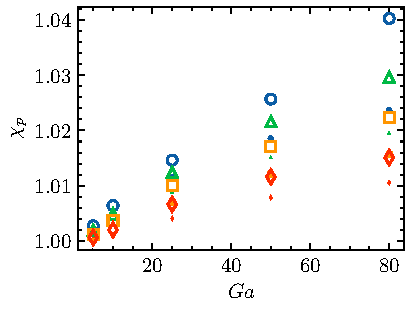
\includegraphics[height = 0.3\textwidth]{image/HOMOGENEOUS_final/PA/chi.pdf}
    \caption{Mean aspect ratio of the droplets $\chi_p$, as a function of the \textit{Galileo} number, and the volume faction $\phi$,  for two different viscosity ratios.  
    The symbols correspond to different volume fraction ($\pmb\bigcirc$) $\phi = 0.01$; ($\pmb\triangle$) $ \phi = 0.05$; ($\pmb\square$) $\phi = 0.1$ ($\pmb\lozenge$) $\phi = 0.2$.
    The hollow symbols correspond to $\lambda = 1$, the small filled symbols to $\lambda = 10$, and the big filled symbols to $\lambda = 0.1$.
    The nearly imperceptible vertical bars on each symbol, represent the standard deviation around the mean.  }
    \label{fig:chi2}
\end{figure}
To verify that the droplets remain on average approximately spherical we plotted in \ref{fig:chi2} the mean aspect ratio $\chi_p$ of the droplets for all of our simulations. 
A rigorous definition of this aspect ratio is given in \citet[Appendix 1]{fintzi2024buoyancy} or \citet{bunner2003effect}. 
At $Bo = 0.5$, the maximum mean droplet deformation $\chi_p$ represents about $5\%$ of deformation for $\lambda = 0.1$, compared to the $2\%$ obtained for $Bo = 0.2$. 
This means that the droplet shape deviates of approximately $5\%$ from their original spherical shape. 


\begin{table}[h!]
    \centering
    \caption{Dimensionless parameter range investigated in this work.}
    \begin{tabular}{|ccccccc|ccc|}
        \hline
        \multicolumn{7}{|c}{Primary parameters} & \multicolumn{3}{||c|}{Secondary parameters}\\ \hline
        \multicolumn{1}{|c|}{$Ga$}                               & \multicolumn{1}{c|}{$Bo$}                   & \multicolumn{1}{c|}{$\phi$} & \multicolumn{1}{c|}{$\lambda$}                    & \multicolumn{1}{c|}{$\zeta$}                & \multicolumn{1}{c|}{$N_b$} & $t_\text{end}$ & \multicolumn{1}{||c|}{$\mathcal{L}/d$} & \multicolumn{1}{c|}{$Re$}  & $We$   \\ \hline
        \multicolumn{1}{|c|}{\multirow{4}{*}{$5\rightarrow 80$}} & \multicolumn{1}{c|}{\multirow{4}{*}{$0.5$}} & \multicolumn{1}{c|}{$1\%$}  & \multicolumn{1}{c|}{\multirow{4}{*}{$10$ $\to$ $0.1$}} & \multicolumn{1}{c|}{\multirow{4}{*}{$0.9$}} & \multicolumn{1}{c|}{$160$} & $400$           & \multicolumn{1}{||c|}{$20$}            & \multicolumn{1}{c|}{$1.1\to 128$} & {$0.03\to 0.95$} \\ 
        \multicolumn{1}{|c|}{}                                   & \multicolumn{1}{c|}{}                       & \multicolumn{1}{c|}{$5\%$}  & \multicolumn{1}{c|}{}                             & \multicolumn{1}{c|}{}                       & \multicolumn{1}{c|}{$800$} & $400$           & \multicolumn{1}{||c|}{$20$}            & \multicolumn{1}{c|}{$0.8\to 106$} &  {$0.02\to 0.67$}\\ 
        \multicolumn{1}{|c|}{}                                   & \multicolumn{1}{c|}{}                       & \multicolumn{1}{c|}{$10\%$} & \multicolumn{1}{c|}{}                             & \multicolumn{1}{c|}{}                       & \multicolumn{1}{c|}{$200$} & $1000$           & \multicolumn{1}{||c|}{$10$}            & \multicolumn{1}{c|}{$0.6\to 87$}&  {$0.01\to 0.47$}\\ 
        \multicolumn{1}{|c|}{}                                   & \multicolumn{1}{c|}{}                       & \multicolumn{1}{c|}{$20\%$} & \multicolumn{1}{c|}{}                             & \multicolumn{1}{c|}{}                       & \multicolumn{1}{c|}{$400$} & $1000$           & \multicolumn{1}{||c|}{$10$}            & \multicolumn{1}{c|}{$0.4\to 69$}&  {$9\cdot 10^{-3}\to 0.31$}\\ \hline
        \end{tabular}
    \label{tab:simulations}
\end{table}
This study presents DNS results with dimensionless parameters in ranges outlined in \ref{tab:simulations}.
In summary, we investigated $5$ \textit{Galileo} number $Ga = 5,10,25,50,80$, $4$ different volume fractions $\phi = 0.01,0.05,0.1,0.2$, and three viscosity ratios $\lambda =0.1,1,10$. 
We recall that $Bo = 0.5$ is the \textit{Bond} number, and $\zeta = 0.9$ is the density ratio defined as $\rho_d/\rho_f$.
This makes a total of $60$ representative simulations.


\subsection{Numerical approximation of the ensemble average}

Following \citet{du2022analysis} we consider ergodicity at all times of the numerical experiment.
Thus, the ensemble average of a quantity $X$ can be approximated by a spatial average $\Xavg{X}$ and a time average $\Tavg{X}$ such that $\avg{X} \approx \Xavg{\Tavg{X}} = \Tavg{\Xavg{X}}$.
Consequently, the ensemble average of a numerical field, $X$, is taken through space and time such that,
\begin{equation}
    \avg{X}
    = \Tavg{\Xavg{X}}
    = \frac{1}{ t_{end} - t_0}\int_{t_0}^{t_{end}} 
    \Xavg{X}(t) dt
\end{equation}
where, 
\begin{equation}
    \Xavg{X}(t)
    = \frac{1}{L^3}\int 
    X(\textbf{x},t) d\textbf{x}
\end{equation}
Where $L$ is the length of one side of the cubic numerical domain.
$t_0$ and $t_{end}$ are the starting time of sampling, and the ending time of sampling which is also the ending time of the simulation, respectively.
In practice, we take $t_0$ such that the simulation reaches a statistically steady regime. 
It has been found that, in general, for the lowest $Ga$, the criterion $t_0 > 50\sqrt{g/d}$ must be respected.  

To compute the phase average of the local phase velocity $\textbf{u}_k^0$, we simply perform an integration over space and time, 
\begin{equation}
    \textbf{u}_k = \frac{1}{\phi_k} \Tavg{\Xavg{\chi_k \textbf{u}_k^0}}
\end{equation}
where the indicator function $\chi_f$ must be understood as its approximation in the DNS, which is the color function used by the CFD code (\url{http://basilisk.fr}). 
Since the homogeneous and statistically steady-state hypotheses are supposed to be true, the mean of the droplet center of mass velocity is equivalent to the dispersed phase averaged velocity, $\textbf{u}_d$.
Thus, we may compute the ensemble average relative velocity used in \ref{eq:C_d} with the trivial operation, 
\begin{equation}
    \textbf{u}_{pf} = 
    \frac{1}{\phi_d} \Tavg{\Xavg{\chi_d \textbf{u}_d^0}}
    - \frac{1}{\phi_f} \Tavg{\Xavg{\chi_f \textbf{u}_f^0}}. 
\end{equation} 
Then, the relative velocity leads us directly to the numerical approximation of the drag force term using \ref{eq:C_d} and \ref{eq:f_p_def}. 

Now that we have all the tools in hand, we present in the next section our generalized drag force model for buoyant droplets of arbitrary viscosity. 